\fe{\subsection{Exercices}}{\subsection{Exercises}}
\label{mecanique_exo}

{\setbeamerfont{framesubtitle}{size=\tiny}
\begin{frame}{\fe{Exercice 1 : poutre avec force suiveuse}{Exercise 1: beam with following force}}
             {\url{https://www-cast3m.cea.fr/index.php?page=exemples&exemple=formation_pasapas_1_initial}}
  \small
  \begin{itemize}
    \item \fe{Poutre en flexion}{Beam bending}\\
    \scriptsize
    \fe{base encastrée, force \tou{perpendiculaire} à la poutre, déplacement "important"}
       {clamped base, force \tou{perpendicular} to the beam, "large" displacement}\\
    \begin{tikzpicture}
      \draw [-,thick] (0,0) -- (0,3);
      \draw [->, red] (0,3) -- (0.5,3) node (force) [right, red] {$F$};
      \draw [-]       (-0.2,0) -- (0.25,0);
      \draw [-]       (-0.2,-0.1) -- (-0.1,0);
      \draw [-]       (-0.1,-0.1) -- (0,0);
      \draw [-]       (0,-0.1) -- (0.1,0);
      \draw [-]       (0.1,-0.1) -- (0.2,0);
    \end{tikzpicture}
    \animategraphics[controls,loop,poster=last,height=3cm]{10}{images/exo/exo_1_deformee.}{01}{21}
    \onslide<2->{
    \begin{textblock*}{10cm}(8cm,-3.5cm)
      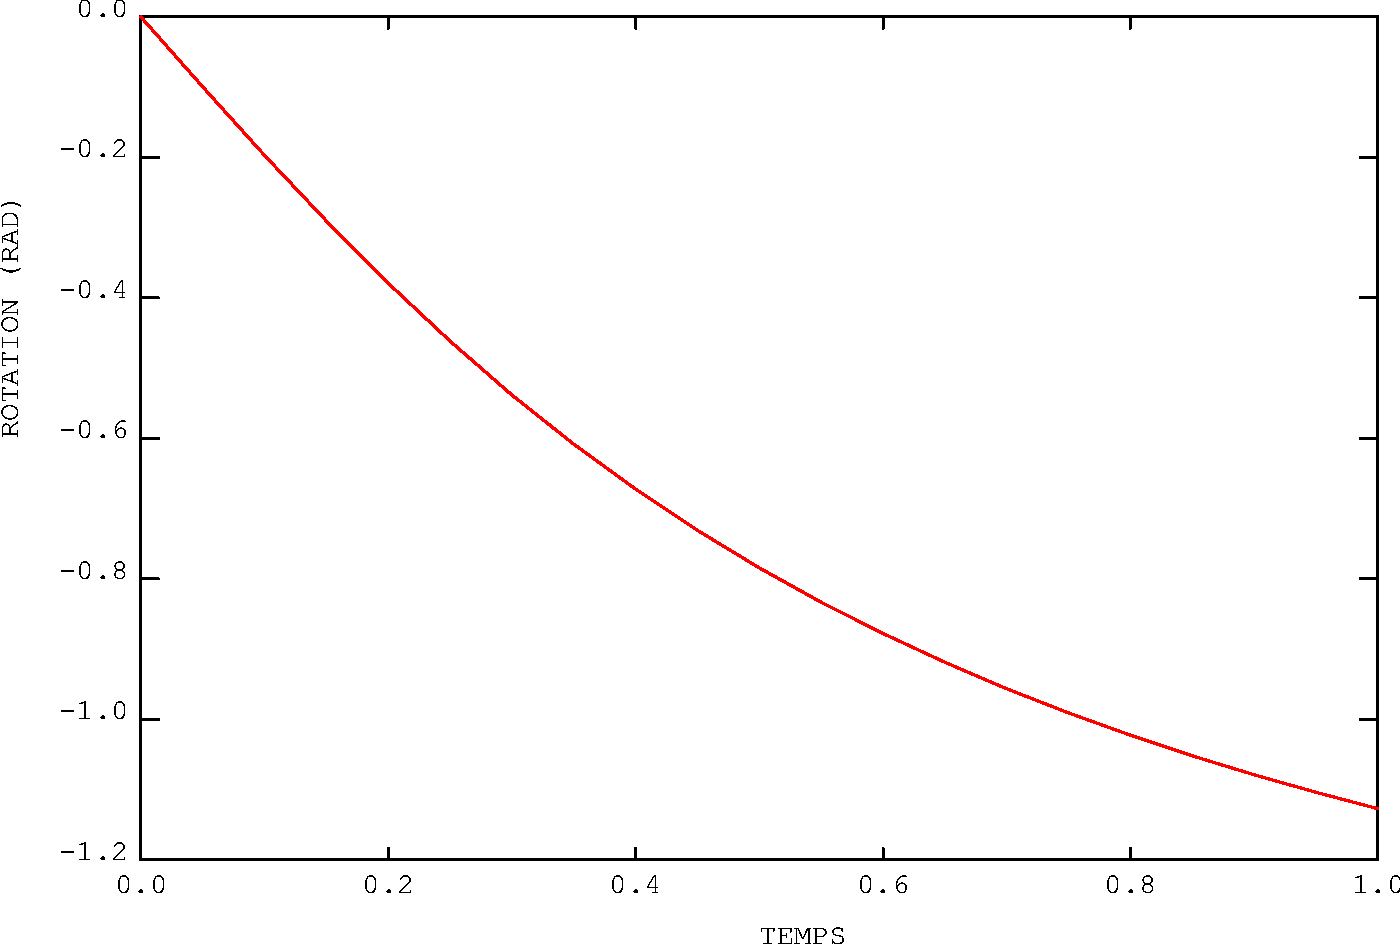
\includegraphics[height=3cm]{images/exo/exo_1_evol}
    \end{textblock*}}
    \normalsize
    \onslide<3->{
    \item \fe{\red{Problème : l'effort est calculé sur la configuration initiale et n'est pas mis à jour}}
             {\red{Problem: the force is calculated on the initial shape and not updated}}
    \item \fe{\green{Objectif : réappliquer l'effort correctement au cours des pas}}
             {\green{Purpose: to correctly apply the force during the calculation}}
    \begin{center}
      \fe{\avous{~À vous de jouer !}}{\avous{~It's up to you!}}
    \end{center}}
  \end{itemize}
\end{frame}
}

{\setbeamerfont{framesubtitle}{size=\tiny}
\begin{frame}{\fe{Exercice 1 : poutre avec force suiveuse}{Exercise 1: beam with following force}}
             {\url{https://www-cast3m.cea.fr/index.php?page=exemples&exemple=formation_pasapas_1_initial}}
  \begin{itemize}
    \item \fe{Quelques objets utiles}{Some useful objects}\\
    \small
    \kw{p2 } \fe{point au sommet de la poutre, où est appliqué la force}{point at the top of the beam, where the force is prescribed}\\
    \kw{ev1} \fe{évolution de l'amplitude de la force à appliquer vs. temps}{force magnitude to be applied as a function of time}
    \normalsize
    \item \fe{Quelques opérateurs utiles}{Some useful operators}\\
    \small
    \kwr{EXTR} \fe{pour extraire des valeurs d'un champ}{to extract values from a field}\\
    \kwr{COS SIN} \fe{pour faire un peu de trigonométrie}{for a bit of trigonometry}\\
    \kwr{IPOL} \fe{pour interpoler l'amplitude de la force à l'instant de calcul}
                  {to interpolate the force magnitude at the current time step}\\
    \kwr{FORC} \fe{pour appliquer une force ponctuelle}{to apply a point force}
    \normalsize
    \item \fe{Quelques indices utiles de la table}{Some useful table indices}\\
    \small
    \kwg{'ESTIMATION'.'DEPLACEMENTS'} \fe{dernier champ de déplacement convergé}{last converged displacement field}
    \kwg{'WTABLE'.'CHARGEMENT'} \fe{chargement courant}{current load}
    \normalsize
  \end{itemize}
\end{frame}
}

\begin{frame}{\fe{Exercice 1 : poutre avec force suiveuse}{Exercise 1: beam with following force}}
             {\fe{Solution avec PERSO1}{Solution with PERSO1}}
  \footnotesize
  \begin{itemize}
    \item \fe{Activer l'option \kwg{'GRANDS\_DEPLACEMENTS'}\\ (équilibre vérifié sur config. déformée)}
             {Use option \kwg{'GRANDS\_DEPLACEMENTS'}\\ (equilibrium verified on the deformed shape)}
    \item \fe{Utiliser la procédure \kwv{PERSO1} \red{(1 appel / pas de temps)} pour mettre à jour la force\\
              sur la configuration déformée au \tou{début du pas (explicite)}}
             {Use procedure \kwv{PERSO1} \red{(1 call / time step)} to update the force on deformed shape\\
              at \tou{beginning of time step (explicit)}}
    \item \fe{Créer un objet CHARGEMEnt et écraser \kwg{'WTABLE' . 'CHARGEMENT'}}
             {Create an load (CHARGEMEnt object) and overwrite \kwg{'WTABLE' . 'CHARGEMENT'}}
  \end{itemize}
  \vspace{4.5cm}
  \scriptsize
  \begin{textblock*}{10cm}(0.3cm,-2.9cm)
    \fe{\emph{Programme principal}}{\emph{Main program}}
    \lstinputlisting[basicstyle=\ttfamily\tiny, language=gibiane, firstline=93, lastline=97]{dgibi/formation_pasapas_1_solution.dgibi}
  \end{textblock*}
  \begin{textblock*}{10cm}(6.3cm,-4.2cm)
    \fe{\emph{\violet{Procédure PERSO1}}}{\emph{\violet{PERSO1 procedure}}}
    \lstinputlisting[basicstyle=\ttfamily\tiny, language=gibiane, firstline=53, lastline=67]{dgibi/formation_pasapas_1_solution.dgibi}
  \end{textblock*}
\end{frame}

\begin{frame}{\fe{Exercice 1 : poutre avec force suiveuse}{Exercise 1: beam with following force}}
             {\fe{Solution avec PERSO1}{Solution with PERSO1}}
  \small
  \begin{itemize}
    \item \fe{Résultats}{Results}\\
    \scriptsize
    \fe{base encastrée, force \tou{perpendiculaire} à la poutre, déplacement "important"}
       {clamped base, force \tou{perpendicular} to the beam, "large" displacement}\\
    \begin{tikzpicture}
      \draw [-,thick] (0,0) -- (0,3);
      \draw [->, red] (0,3) -- (0.5,3) node (force) [right, red] {$F$};
      \draw [-]       (-0.2,0) -- (0.25,0);
      \draw [-]       (-0.2,-0.1) -- (-0.1,0);
      \draw [-]       (-0.1,-0.1) -- (0,0);
      \draw [-]       (0,-0.1) -- (0.1,0);
      \draw [-]       (0.1,-0.1) -- (0.2,0);
    \end{tikzpicture}
    \hspace{0.9cm}
    \animategraphics[controls,loop,poster=last,height=3cm]{10}{images/exo/exo_1_solu_deformee.}{01}{21}
    \begin{textblock*}{10cm}(8cm,-3.5cm)
      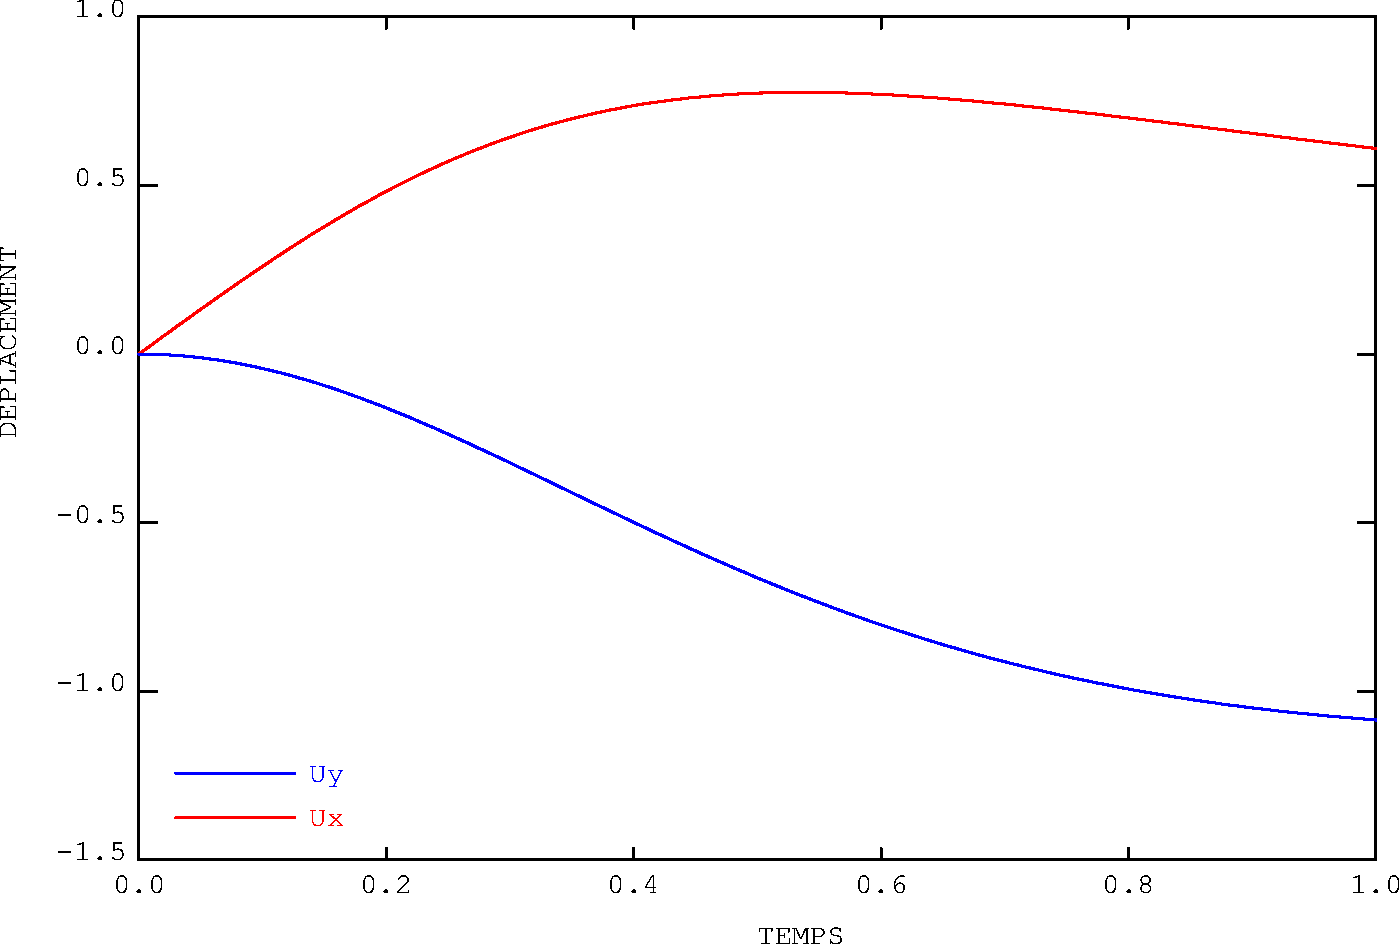
\includegraphics[height=3cm]{images/exo/exo_1_solu_evol}
    \end{textblock*}
    \normalsize
  \end{itemize}
\end{frame}

\begin{frame}{\fe{Exercice 1 : poutre avec force suiveuse}{Exercise 1: beam with following force}}
             {\fe{Solution (bis) avec CHARMECA}{Solution (bis) with CHARMECA}}
  \footnotesize
  \begin{itemize}
    \item \fe{Idem mais avec la procédure \kwv{CHARMECA}, pour mettre à jour la force\\
              sur la configuration déformée au \tou{début du pas (explicite)}}
             {Idem but with the \kwv{CHARMECA} procedure, to update the force on deformed shape\\
              at \tou{beginning of time step (explicit)}}
    \item \fe{Pas besoin de CHARGEMEnt initial}{No need for initial load (CHARGEMEnt object)}
    \item \fe{\red{Plus long (1 appel / itération / pas de temps)} et \green{résultats identiques}}
             {\red{Longer (1 call / each iteration / time step)} and \green{results are identical}}
  \end{itemize}
  \vspace{4.5cm}
  \scriptsize
  \begin{textblock*}{10cm}(0.3cm,-2.9cm)
    \fe{\emph{Programme principal}}{\emph{Main program}}
    \lstinputlisting[basicstyle=\ttfamily\tiny, language=gibiane, firstline=143, lastline=149]{dgibi/formation_pasapas_1_solution.dgibi}
  \end{textblock*}
  \begin{textblock*}{10cm}(6.3cm,-4.3cm)
    \fe{\emph{\violet{Procédure CHARMECA}}}{\emph{\violet{CHARMECA procedure}}}
    \lstinputlisting[basicstyle=\ttfamily\tiny, language=gibiane, firstline=69, lastline=83]{dgibi/formation_pasapas_1_solution.dgibi}
  \end{textblock*}
\end{frame}

\begin{frame}{\fe{Exercice 1 : poutre avec force suiveuse}{Exercise 1: beam with following force}}
             {\fe{Solution (ter) avec CHARMECA}{Solution (ter) with CHARMECA}}
  \footnotesize
  \begin{itemize}
    \item \fe{Idem mais avec la procédure \kwv{CHARMECA}, pour mettre à jour la force\\
              sur la configuration déformée à la \tou{fin du pas (implicite)}}
             {Idem but with the \kwv{CHARMECA} procedure, to update the force on deformed shape\\
              at the \tou{end of time step (implicit)}}
    \item \fe{Attention : peut être instable !}{Watch out: can become unstable!}
  \end{itemize}
  \vspace{4.5cm}
  \scriptsize
  \begin{textblock*}{10cm}(0.3cm,-2.9cm)
    \fe{\emph{Programme principal}}{\emph{Main program}}
    \lstinputlisting[basicstyle=\ttfamily\tiny, language=gibiane, firstline=143, lastline=149]{dgibi/formation_pasapas_1_solution.dgibi}
  \end{textblock*}
  \begin{textblock*}{10cm}(6.3cm,-4.4cm)
    \fe{\emph{\violet{Procédure CHARMECA}}}{\emph{\violet{CHARMECA procedure}}}
    \lstinputlisting[basicstyle=\ttfamily\tiny, language=gibiane, firstline=151, lastline=168]{dgibi/formation_pasapas_1_solution.dgibi}
  \end{textblock*}
\end{frame}
